% !TeX root = ../main.tex

\section{Initialization Study}
\label{sec:abs1-init}

% ------------------------------------------------------------------

\subsection*{Study Motivation}

This experiment tests the most fundamental implementation of prototype surface learning theory: a single linear neuron followed by an absolute-value activation, $y = |w^{\mathsf{T}}x + b|$. As detailed in Section~\ref{sec:abs1-model-data}, this architecture directly implements a scaled distance metric from input points to a learned hyperplane, making it the minimal viable test of the theory's core mechanism.

The absolute-value activation is designed to solve XOR by learning a prototype surface that intersects the points assigned to the zero class (the ``False'' XOR outputs). According to the theory, the network should position its hyperplane $w^{\mathsf{T}}x + b = 0$ to pass through these prototype points, while placing the ``True'' class points at a distance of $\sqrt{2}$.

We systematically test five initialization strategies to understand how different starting weight scales affect this fundamental learning process. Since the analytical optimum is known (Section~\ref{sec:abs1-model-data}), we can directly validate whether empirical learning recovers the theoretically predicted geometry regardless of initialization.

This experiment serves multiple purposes: it provides geometric validation of prototype surface learning, establishes our experimental methodology and analysis framework, and creates a performance baseline for comparison with more complex architectures in subsequent chapters. The insights gained about initialization effects will directly inform strategies for training the multi-neuron models that follow.RetryClaude can make mistakes. Please double-check responses.

% ------------------------------------------------------------------

\subsection*{Study Design}

\paragraph{Model Architecture}
All experiments use the single absolute-value neuron defined in Section~\ref{sec:abs1-model-data}: $\hat{y}(x) = |w^{\mathsf{T}}x + b|$ with $w \in \mathbb{R}^2$ and $b \in \mathbb{R}$. The model is trained on the centered XOR dataset with mean-squared error loss.

\paragraph{Initialization Variants}
We test five weight initialization schemes, each applied to 50 independent runs:
\begin{itemize}
   \item \textbf{Tiny}: $w \sim \mathcal{N}(0, 0.1^2)$ -- small initial weights
   \item \textbf{Normal}: $w \sim \mathcal{N}(0, 0.5^2)$ -- standard Gaussian initialization  
   \item \textbf{Xavier}: $w \sim \mathcal{N}(0, 1/n_{\text{in}})$ -- Xavier/Glorot initialization
   \item \textbf{Kaiming}: $w \sim \mathcal{N}(0, 2/n_{\text{in}})$ -- He/Kaiming initialization
   \item \textbf{Large}: $w \sim \mathcal{N}(0, 4.0^2)$ -- large initial weights
\end{itemize}
All bias parameters are initialized to zero across variants.

\paragraph{Training Protocol}
Each run uses identical training conditions: Adam optimizer ($\text{lr}=0.01$, $\beta=(0.9, 0.99)$), MSE loss, and a maximum of 1000--2000 epochs depending on the variant. Training terminates early when the loss drops below $\varepsilon = 10^{-7}$.

% ------------------------------------------------------------------

\subsection*{Success Metrics}

\begin{table}[ht]
\centering
\caption{Number of runs (out of 50) achieving each discrete accuracy level on the centred XOR dataset.  All variants ultimately attain $100\,\%$ accuracy.}
\label{tab:abs1-init-accuracy}
\begin{tabular}{lccccc}
\toprule
\multirow{2}{*}{Init} & \multicolumn{5}{c}{Accuracy level}\\
\cmidrule(lr){2-6}
& 0\% & 25\% & 50\% & 75\% & 100\% \\
\midrule
Tiny    & 0 & 0 & 0 & 0 & 50 \\
Normal  & 0 & 0 & 0 & 0 & 50 \\
Xavier  & 0 & 0 & 0 & 0 & 50 \\
Kaiming & 0 & 0 & 0 & 0 & 50 \\
Large   & 0 & 0 & 0 & 0 & 50 \\
\bottomrule
\end{tabular}
\end{table}

\begin{table}[ht]
\centering
\caption{Mean final loss and range across runs.}
\label{tab:abs1-init-loss}
\begin{tabular}{lccc}
\toprule
Init & Mean & Min & Max \\
\midrule
Tiny    & $1.32\times10^{-7}$ & $1.6\times10^{-8}$ & $3.0\times10^{-7}$ \\
Normal  & $7.81\times10^{-8}$ & $2.6\times10^{-9}$ & $7.6\times10^{-7}$ \\
Xavier  & $1.11\times10^{-7}$ & $2.4\times10^{-11}$ & $2.0\times10^{-7}$ \\
Kaiming & $7.06\times10^{-8}$ & $3.1\times10^{-10}$ & $1.0\times10^{-6}$ \\
Large   & $7.37\times10^{-8}$ & $1.4\times10^{-8}$ & $8.4\times10^{-8}$ \\
\bottomrule
\end{tabular}
\end{table}

All initialization schemes achieve perfect classification success, with every run converging to $100\,\%$ XOR accuracy. This uniform success validates the theoretical prediction that the analytic optimum is reachable from any weight orientation, demonstrating the robustness of the single absolute-value architecture and the convex-like properties of its loss landscape.

The final loss distributions reveal additional patterns in solution quality. Large initialization produces the most consistent final precision (range: $1.4 \times 10^{-8}$ to $8.4 \times 10^{-8}$), while Xavier achieves the highest precision in individual runs (down to $2.4 \times 10^{-11}$) but with greater variance. All variants terminate near machine precision, confirming that the absolute-value activation creates a smooth optimization surface once the correct sign pattern is established.

This success uniformity establishes a crucial baseline: initialization choice affects only optimization efficiency, not final effectiveness. Unlike the multi-neuron ReLU experiments in later chapters where success rates drop dramatically, the hard-coded symmetry of the absolute-value function eliminates local minima and convergence failures. This creates an ideal controlled setting for studying initialization effects on learning dynamics without confounding factors from variable success rates.

% ------------------------------------------------------------------

\subsection*{Learning Dynamics}

\begin{table}[ht]
\centering
\caption{Epochs to reach $\mathcal L<10^{-7}$ (percentiles over 50 runs).}
\label{tab:abs1-init-epochs}
\begin{tabular}{lccccc}
\toprule
Init & 0\,\% & 25\,\% & 50\,\% & 75\,\% & 100\,\% \\
\midrule
Tiny    & 75  & 141 & 147 & 154 & 166 \\
Normal  & 76  & 127 & 146 & 164 & 297 \\
Xavier  & 62  & 122 & 151 & 234 & 449 \\
Kaiming & 61  & 139 & 198 & 266 & 548 \\
Large   & 154 & 527 & 671 & 878 & 1670 \\
\bottomrule
\end{tabular}
\end{table}

\begin{table}[ht]
\centering
\caption{Median angle (in degrees) between initial and final weights, median norm ratio $\lVert W_{\text{init}}\rVert / \lVert W_{\text{final}}\rVert$, and median epochs to convergence.}
\label{tab:abs1-init-angle-norm}
\begin{tabular}{lccc}
\toprule
Init & Angle (median) & Norm ratio (median) & Epochs (median) \\
\midrule
Tiny    & 22.0 & 0.16 & 147 \\
Normal  & 23.2 & 0.81 & 146 \\
Xavier  & 22.1 & 1.33 & 151 \\
Kaiming & 22.0 & 1.63 & 198 \\
Large   & 22.0 & 6.54 & 671 \\
\bottomrule
\end{tabular}
\end{table}

Convergence time grows monotonically with initial weight scale, spanning nearly an order of magnitude from Tiny (median 147 epochs) to Large (median 671 epochs). This dramatic timing difference suggests that weight magnitude is the primary factor governing optimization speed.

The weight evolution analysis reveals potential relationships between initialization geometry and convergence time. The angle between initial and final weights represents the rotational correction needed, since the optimal XOR solutions lie at $\pm45\circ$ in weight space. Most initializations require similar rotational adjustments (median $\sim22\circ$), suggesting that random initializations start at relatively consistent angular distances from the optimal solutions.

The norm ratio shows a clearer relationship with convergence speed. Large initialization requires the most dramatic magnitude adjustment (ratio 6.54), corresponding to the slowest median convergence (671 epochs). Detailed analysis reveals hints of systematic relationships: for Large initialization, convergence time increases monotonically with the required norm adjustment, ranging from 203 epochs (smallest adjustments) to 1316 epochs (largest adjustments). Similar but weaker patterns appear for other initialization schemes.

However, these relationships are complex and inconsistent across initialization types. While weight magnitude appears to dominate optimization dynamics, the interaction between initial orientation and scale effects requires deeper investigation. The current analysis suggests that prediction of convergence time from initialization geometry is possible but would require more sophisticated analysis.

% ------------------------------------------------------------------

\subsection*{Geometric Analysis}

The analytic optimum (Section~\ref{sec:abs1-model-data}) predicts that learning should anchor the prototype surface to the two \textbf{False} points and place the \textbf{True} points at Euclidean distance $\sqrt{2}$. We validate this prediction through two complementary geometric analyses.

\paragraph{Distance Pattern Analysis}
For each run we compute $(d_{\text{False}}, d_{\text{True}})$, the mean distance from each class to the learned hyperplane $w^{\mathsf{T}}x + b = 0$. This tests whether the network achieves the predicted functional relationship: anchoring the decision boundary to one class while calibrating weight magnitude to produce the correct output for the other class.

\begin{table}[ht]
\centering
\caption{Distance patterns from data points to learned hyperplanes (50 runs per initializer). All variants achieve identical geometric relationships.}
\label{tab:abs1-distance-clusters}
\begin{tabular}{lccc}
\toprule
Init & Class 0 Distance & Class 1 Distance & \# Distance Clusters \\
\midrule
Tiny    & $0.00 \pm 0.00$ & $1.41 \pm 0.00$ & 1 \\
Normal  & $0.00 \pm 0.00$ & $1.41 \pm 0.00$ & 1 \\
Xavier  & $0.00 \pm 0.00$ & $1.41 \pm 0.00$ & 1 \\
Kaiming & $0.00 \pm 0.00$ & $1.41 \pm 0.00$ & 1 \\
Large   & $0.00 \pm 0.00$ & $1.41 \pm 0.00$ & 1 \\
\bottomrule
\end{tabular}
\end{table}

All initialization schemes produce identical distance patterns. The False points lie exactly on the hyperplane ($d_{\text{False}} = 0$), confirming that the network anchors its decision boundary to this class. The True points are positioned at distance $1.41 \approx \sqrt{2}$, precisely matching the theoretical prediction. The tight clustering demonstrates that prototype surface learning produces a consistent functional relationship regardless of initialization.

\paragraph{Solution Structure Analysis}
We cluster the learned parameter vectors $(w_1, w_2, b)$ using DBSCAN to reveal how many distinct geometric solutions can achieve the required distance pattern.

\begin{table}[ht]
\centering
\caption{Weight space clustering reveals the structure of geometric solutions (50 runs per initializer). Numbers in parentheses show cluster sizes.}
\label{tab:abs1-weight-clusters}
\begin{tabular}{lcc}
\toprule
Init & \# Weight Clusters & Cluster Centroids \\
\midrule
Tiny    & 2 (27/23) & $(0.5, -0.5, 0)$ and $(-0.5, 0.5, 0)$ \\
Normal  & 2 (30/20) & $(0.5, -0.5, 0)$ and $(-0.5, 0.5, 0)$ \\
Xavier  & 2 (27/23) & $(0.5, -0.5, 0)$ and $(-0.5, 0.5, 0)$ \\
Kaiming & 2 (27/23) & $(0.5, -0.5, 0)$ and $(-0.5, 0.5, 0)$ \\
Large   & 2 (27/23) & $(0.5, -0.5, 0)$ and $(-0.5, 0.5, 0)$ \\
\bottomrule
\end{tabular}
\end{table}

Every initialization discovers exactly two sign-symmetric parameter clusters, representing mirror-image hyperplane orientations that achieve identical distance relationships. The solution space is highly constrained: rather than a continuous manifold of possibilities, only two discrete geometric configurations satisfy the prototype surface requirements.

\begin{figure}[ht]
 \centering
 \begin{subfigure}{0.46\textwidth}
   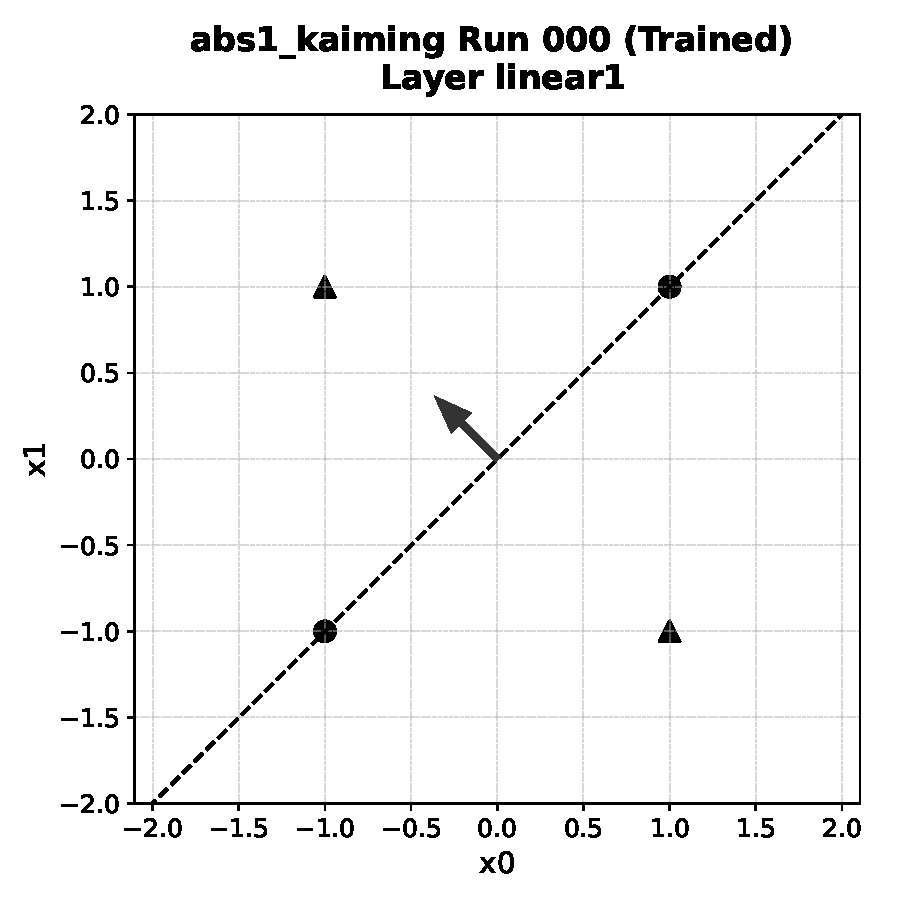
\includegraphics[width=\linewidth]{abs1/figs/kaiming_run000.pdf}
   \caption{Solution 1: $(0.5, -0.5, 0)$}
 \end{subfigure}\hfill
 \begin{subfigure}{0.46\textwidth}
   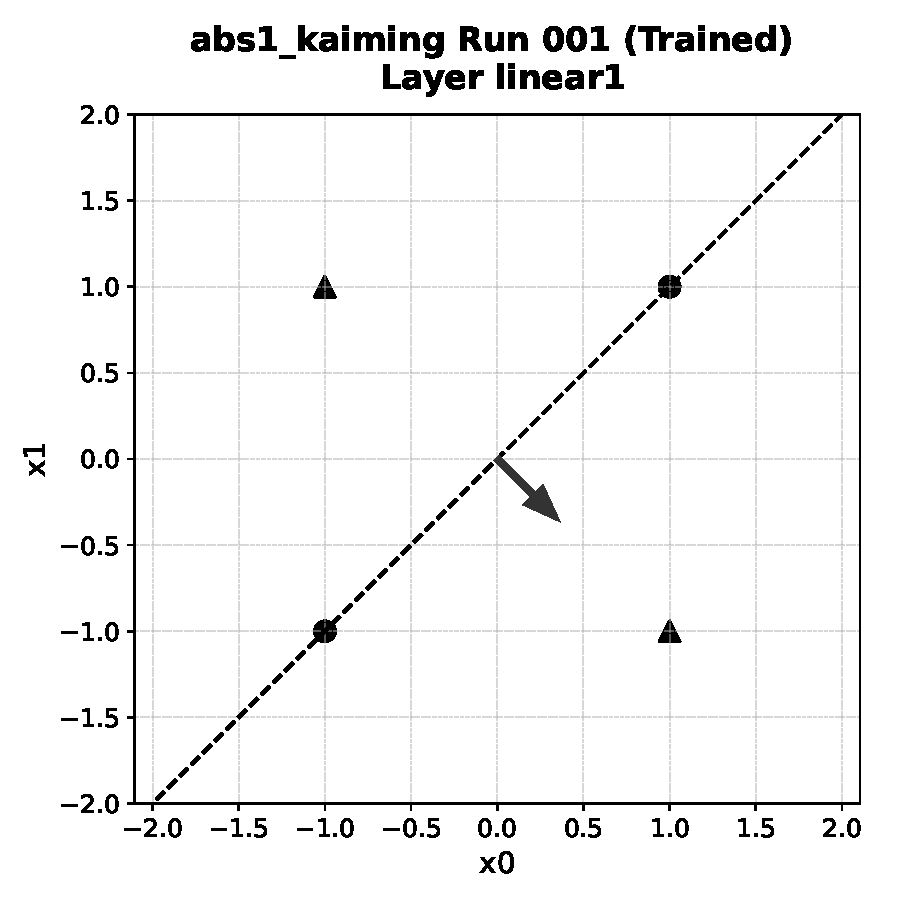
\includegraphics[width=\linewidth]{abs1/figs/kaiming_run001.pdf}
   \caption{Solution 2: $(-0.5, 0.5, 0)$}
 \end{subfigure}
 \caption{Two mirror-symmetric prototype surfaces from Kaiming initialization. Both hyperplanes (dashed lines) pass through the False points ($\bullet$) and position True points ($\blacktriangle$) at distance $\sqrt{2}$. Arrows indicate hyperplane normal directions.}
 \label{fig:abs1-hyperplanes}
\end{figure}

Figure~\ref{fig:abs1-hyperplanes} visualizes the two solution clusters. Despite opposite hyperplane orientations (different arrow directions), both achieve identical functional relationships: the hyperplane passes through the False points and places the True points at the calibrated distance needed for correct outputs.

\paragraph{Theoretical Validation}
These results provide direct empirical validation of prototype surface learning theory. The network learns by positioning its zero-level set to intersect the prototype class (False points) while calibrating weight magnitude so the non-prototype class (True points) produces the target activation. The consistent geometry across all initializations demonstrates that this mechanism represents a fundamental attractor in the learning dynamics, not an artifact of specific training conditions.

% ------------------------------------------------------------------

\subsection*{Study Discussion}

This experiment demonstrates the remarkable robustness of the single absolute-value neuron architecture, achieving $100\,\%$ XOR classification success across all initialization schemes. This universal success stems from the analytical tractability of the model: with a known closed-form optimum, the loss landscape contains no local minima that can trap the optimizer. The hard-coded symmetry of the absolute-value activation eliminates the coordination challenges that plague more complex architectures, creating an ideal baseline for prototype surface learning.

The learning dynamics reveal intriguing relationships between initialization geometry and convergence speed. While convergence time scales monotonically with weight magnitude, our analysis hints at more subtle correlations between parameter distance metrics (angular and magnitude changes) and training epochs. However, these relationships remain incompletely understood and require more sophisticated modeling to quantify precisely. The consistent $\sim22^\circ$ median rotation across initializations suggests fundamental geometric constraints in how random orientations transition to the optimal XOR-solving hyperplane.

The geometric analysis provides direct empirical validation of prototype surface learning theory. Every successful run learns by anchoring its hyperplane to intersect the "False" class points (zero-output targets) while calibrating weight magnitude to position the "True" class at the precise distance needed for correct activation. This demonstrates negative representation learning: the network encodes class membership through the zero-level set rather than positive activations. Importantly, this mechanism is label-independent—if we reversed the 0/1 class assignments, the network would anchor to the other two points, confirming that the underlying geometric principle is general.

Several anomalies warrant future investigation. Large initialization paradoxically achieves the lowest final loss ($7.37 \times 10^{-8}$ mean) despite requiring the most training epochs, suggesting dramatic single-step loss reductions that bypass our stopping threshold. This implies complex optimization dynamics that merit deeper analysis as we scale to more sophisticated architectures.

Given the similar geometric outcomes across initialization schemes, we find no compelling advantage for any particular strategy. Consequently, we will use Kaiming initialization as our default for subsequent experiments, providing consistency with standard deep learning practice while maintaining the geometric reliability demonstrated here.

These results establish the single absolute-value neuron as an ideal prototype surface learning baseline. The next challenge is testing how these principles extend to multi-neuron architectures where symmetry must be learned rather than hard-coded. The transition from deterministic success to the coordination challenges of independent ReLU neurons will reveal which aspects of prototype surface learning are fundamental versus artifacts of this simplified setting.
